%\addcontentsline{toc}{chapter}{Development Process}
\chapter{Design}

% You should concentrate on the more important aspects of the design. It is essential that an overview is presented before going into detail. As well as describing the design adopted it must also explain what other designs were considered and why they were rejected.

% The design should describe what you expected to do, and might also explain areas that you had to revise after some investigation.

% Typically, for an object-oriented design, the discussion will focus on the choice of objects and classes and the allocation of methods to classes. The use made of reusable components should be described and their source referenced. Particularly important decisions concerning data structures usually affect the architecture of a system and so should be described here.

% How much material you include on detailed design and implementation will depend very much on the nature of the project. It should not be padded out. Think about the significant aspects of your system. For example, describe the design of the user interface if it is a critical aspect of your system, or provide detail about methods and data structures that are not trivial. Do not spend time on long lists of trivial items and repetitive descriptions. If in doubt about what is appropriate, speak to your supervisor.
 
% You should also identify any support tools that you used. You should discuss your choice of implementation tools - programming language, compilers, database management system, program development environment, etc.

% Some example sub-sections may be as follows, but the specific sections are for you to define. 

\section{Overall Architecture}
The design of the application evolved over time due to being developed using agile methodologies. This meant that each step had an initial design and was built upon every time a new feature was added, being refactored along the way. There were a number of prototypes made during the course of the project's development, and this chapter will discuss the design of the end product, and go into detail where the design may have been previously different.

The resulting application evolved into a web service, with a Model View Controller (MVC) framework and resources structured for maintainability. Following XPs guidelines, at each step of the way the applications design was made as such to be the simplest yet most maintainable it could be through refactoring, cutting down on duplicate code, structured logically and choosing smart data structures and Objects to represent aspects of the application and quality results.

\subsection{Choice of technologies}
At the beginning of the application, I felt that the application should be programmed in a language that would be able to be ported across multiple platforms for used by anybody who wished to use it. Additionally to this, I wanted to have ways of representing the components of my application as Objects and would need some way of presenting a UI to the user, even if my initial application would only output command line results, in order to follow the XP value of Simplicity (YAGNI - ``You Ain't Gonna Need It'', until you do).

For this reason, I selected to develop my application using Java to begin with as it filled the criteria of being Object Oriented and was portable through using the JVM on different operating systems. I resolved that I would select a UI package to present the report of my results once some of the core functionality had been implemented. I considered instead using Ruby or C++, but due to my familiarity with Java I believed it would be a better choice to stick with what I knew. At this point, I did not consider having the application as a web service, and so using Ruby with Rails was not something I had thought of.

As the application developed and I started reading in files and outputting results from the GC Content process, I found that I was having a hard time finding a quickly usable GUI I could work with for Java to display the results in a way that I wanted. It was at this point I started considering a technology change to Ruby on Rails until Sion Griffiths, a peer of mine, suggested I could keep my application in Java and turn it into a web service using Spring Framework\cite{spring}, and using Spring Boot to easily set up the application with Tomcat for me\cite{springboot}. This seemed like the perfect solution to my problem, allowing me to generate my charts and results using HTML5, JavaScript and HTML5 Canvas, along with JavaScript libraries such as Plotly.js.

The conversion to Java Spring was not a painful one, and only involved setting up a new Maven project and declaring it to run as a Spring application in the pom.xml file, then copying over my previous code and structure into the new project. From there I could deploy the application as a web server using Tomcat and I was back to my previous position of working out a User Interface solutions. Thankfully, there is a package called Thymeleaf\cite{thymeleaf} that works with Spring to allow access to Objects from within the Model of the Java code (placed there by the Controller) using the View dynamically as the View is generated through HTML templates and fragments.

\begin{figure}[H]
	\centering
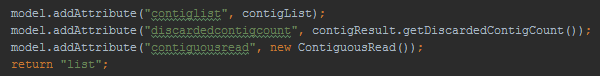
\includegraphics[width=1\textwidth]{images/addingtomodel}
\caption{Adding an object to the Model via the Controller to be accessed in the View. The View here is `list', which is a Thymeleaf template that will dynamically build the page using the data from the Model added here.}
\end{figure}

On top of using Thymeleaf for accessing data put into the Model, it has the additional benefit of using fragments that can be imported into different HTML templates. This design choice made it so I was able to cut down on writing duplicates of code. For example, I wrote the header and footer of the UI design in a Thymeleaf HTML fragment, and then on each page just needed to call one line in order to import it into that page, rather than built the entire thing again. An extra benefit to this is that it allowed me to keep the HTML templates clean and easier to maintain by reducing their size and separating out different aspects of the UI. Having the header, footer and a number of forms in Thymeleaf HTML templates meant that these sections could be edited without impacting any page they are imported into.

\begin{figure}[H]
	\centering
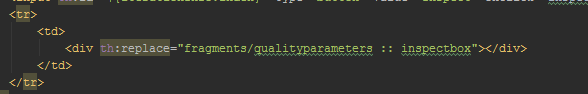
\includegraphics[width=1\textwidth]{images/thymeleafinsert1}
\caption{Including a thymeleaf fragment in a page. You can see how the call is made from one `th:replace' with the name of the html fragment file and then the fragment to be included from that file, in this case `inspectbox'.}
\end{figure}
\begin{figure}[H]
\centering
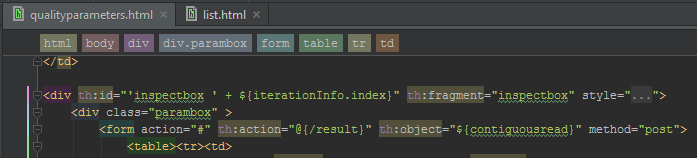
\includegraphics[width=1\textwidth]{images/thymeleafinsert2}
\caption{Including a thymeleaf fragment in a page. This is the declaration of the fragment being included in the previous figure, declared as such through `th:fragment'.}
\end{figure}

For the GUI itself, I elected to use Plotly.js\cite{plotly} for representing my GC content charts for the level of detail and control it gives a user over inspecting charts, large and small, that worked no matter what GC window size the user selected. For the ORF Locations frames charts I wrote my own code using JavaScript and displayed it with HTML5 Canvas, as it allowed me control over what should be shown depending what a user clicks upon and I could work with the data from the Model in ways I saw fit.

\subsection{MVC Framework}
As I was building an application with a GUI, the application was built using a Model View Controller framework design, separating out the components into their different types. This helped the separation of code and responsibilities. The class diagrams presented in this chapter are based on the final product design and based on a page per page view from the UI and what classes are used on the HTML request of that page.

\begin{figure}[H]
\centering
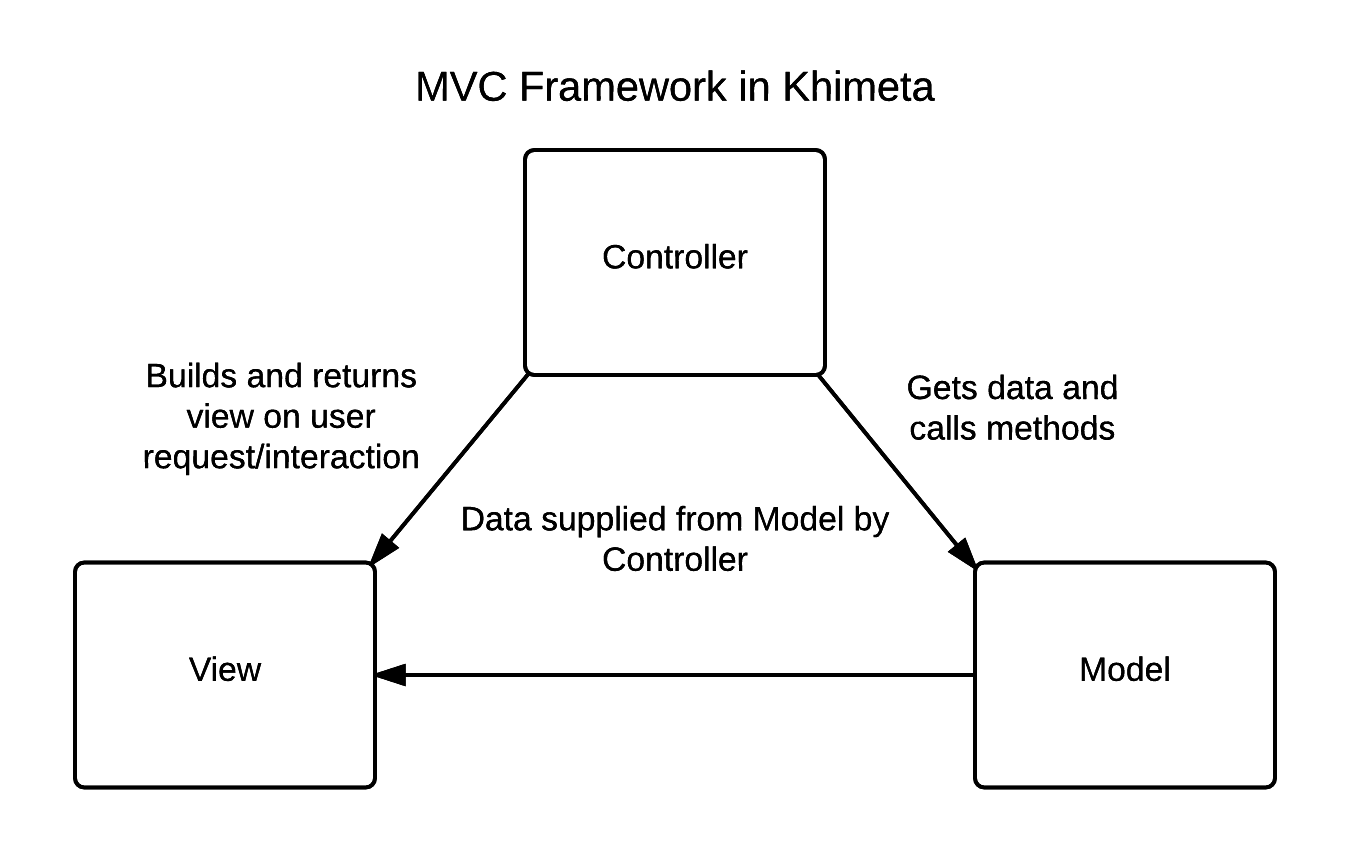
\includegraphics[width=0.9\textwidth]{images/mvcframework}
\caption{The MVC framework the application is designed upon. The data flows between the Model and the View via the Controller, based on the user requests and interaction.}
\end{figure}

\subsubsection{Model}
The Model was designed to contain the data and methods for processing a users input. This contains the data structures and objects for handling a users data as they traverse from page to page of the view. I designed the Model in a way that certain objects would be Bean objects (classes with getters and setters for their properties) that could be accessed by the View in the way that Thymeleaf required.

\begin{figure}[H]
\centering
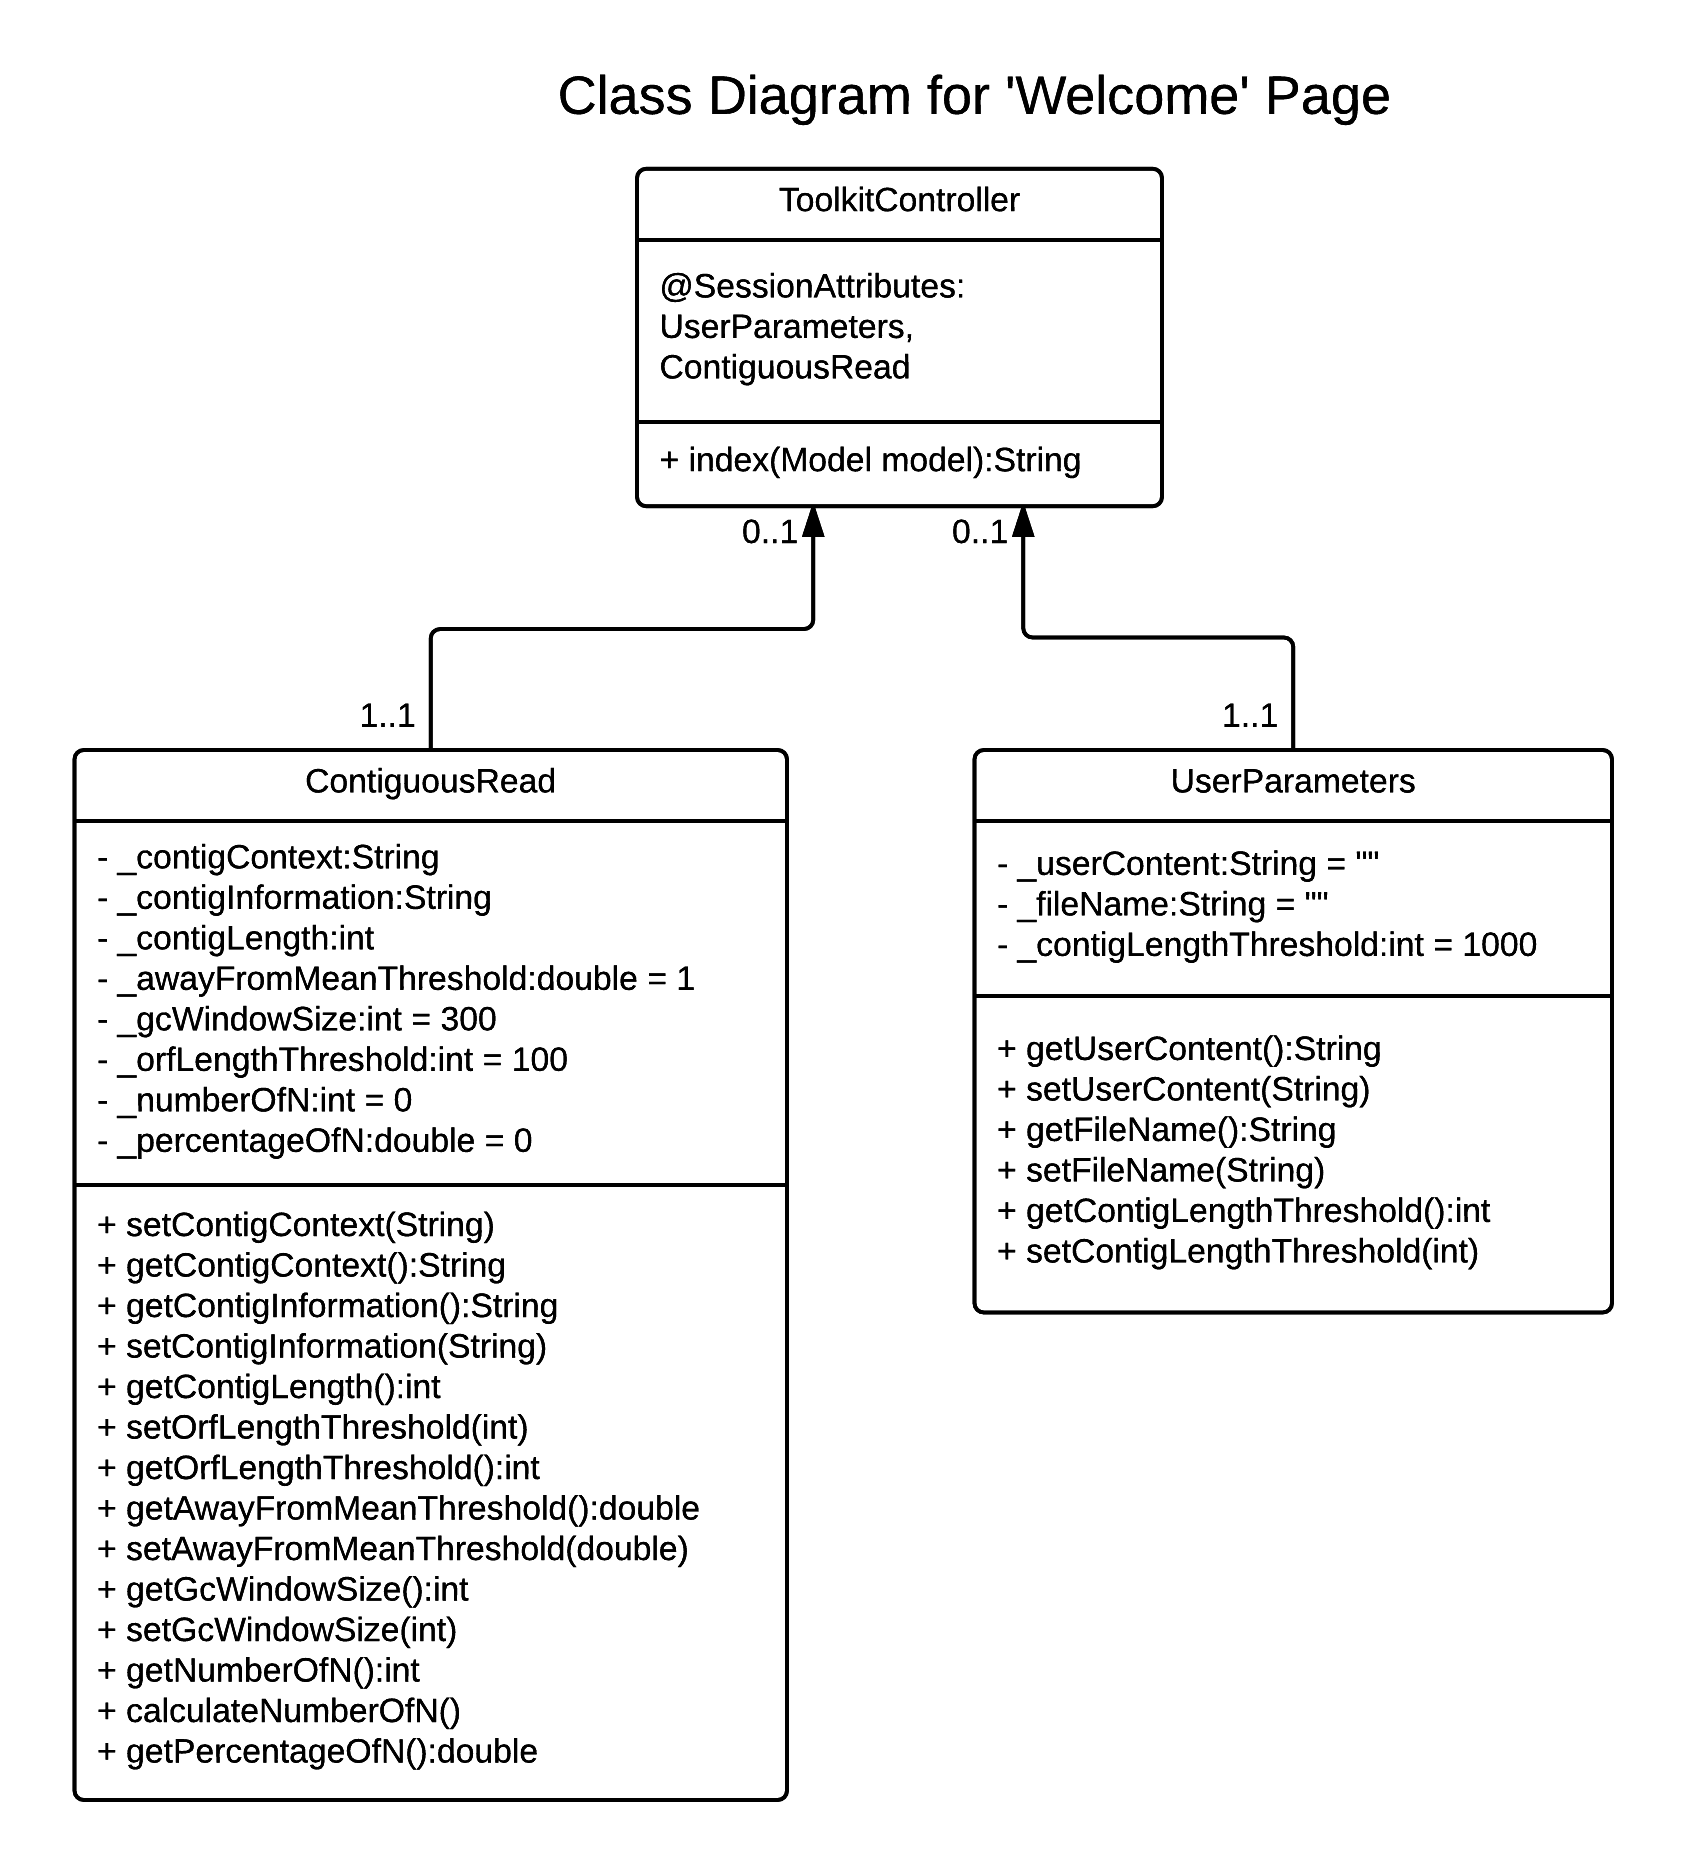
\includegraphics[width=0.7\textwidth]{images/umlwelcomepage}
\caption{Class diagram for the `Welcome Page', and what classes are used upon a Request for the page.}
\end{figure}

\begin{figure}[H]
\centering
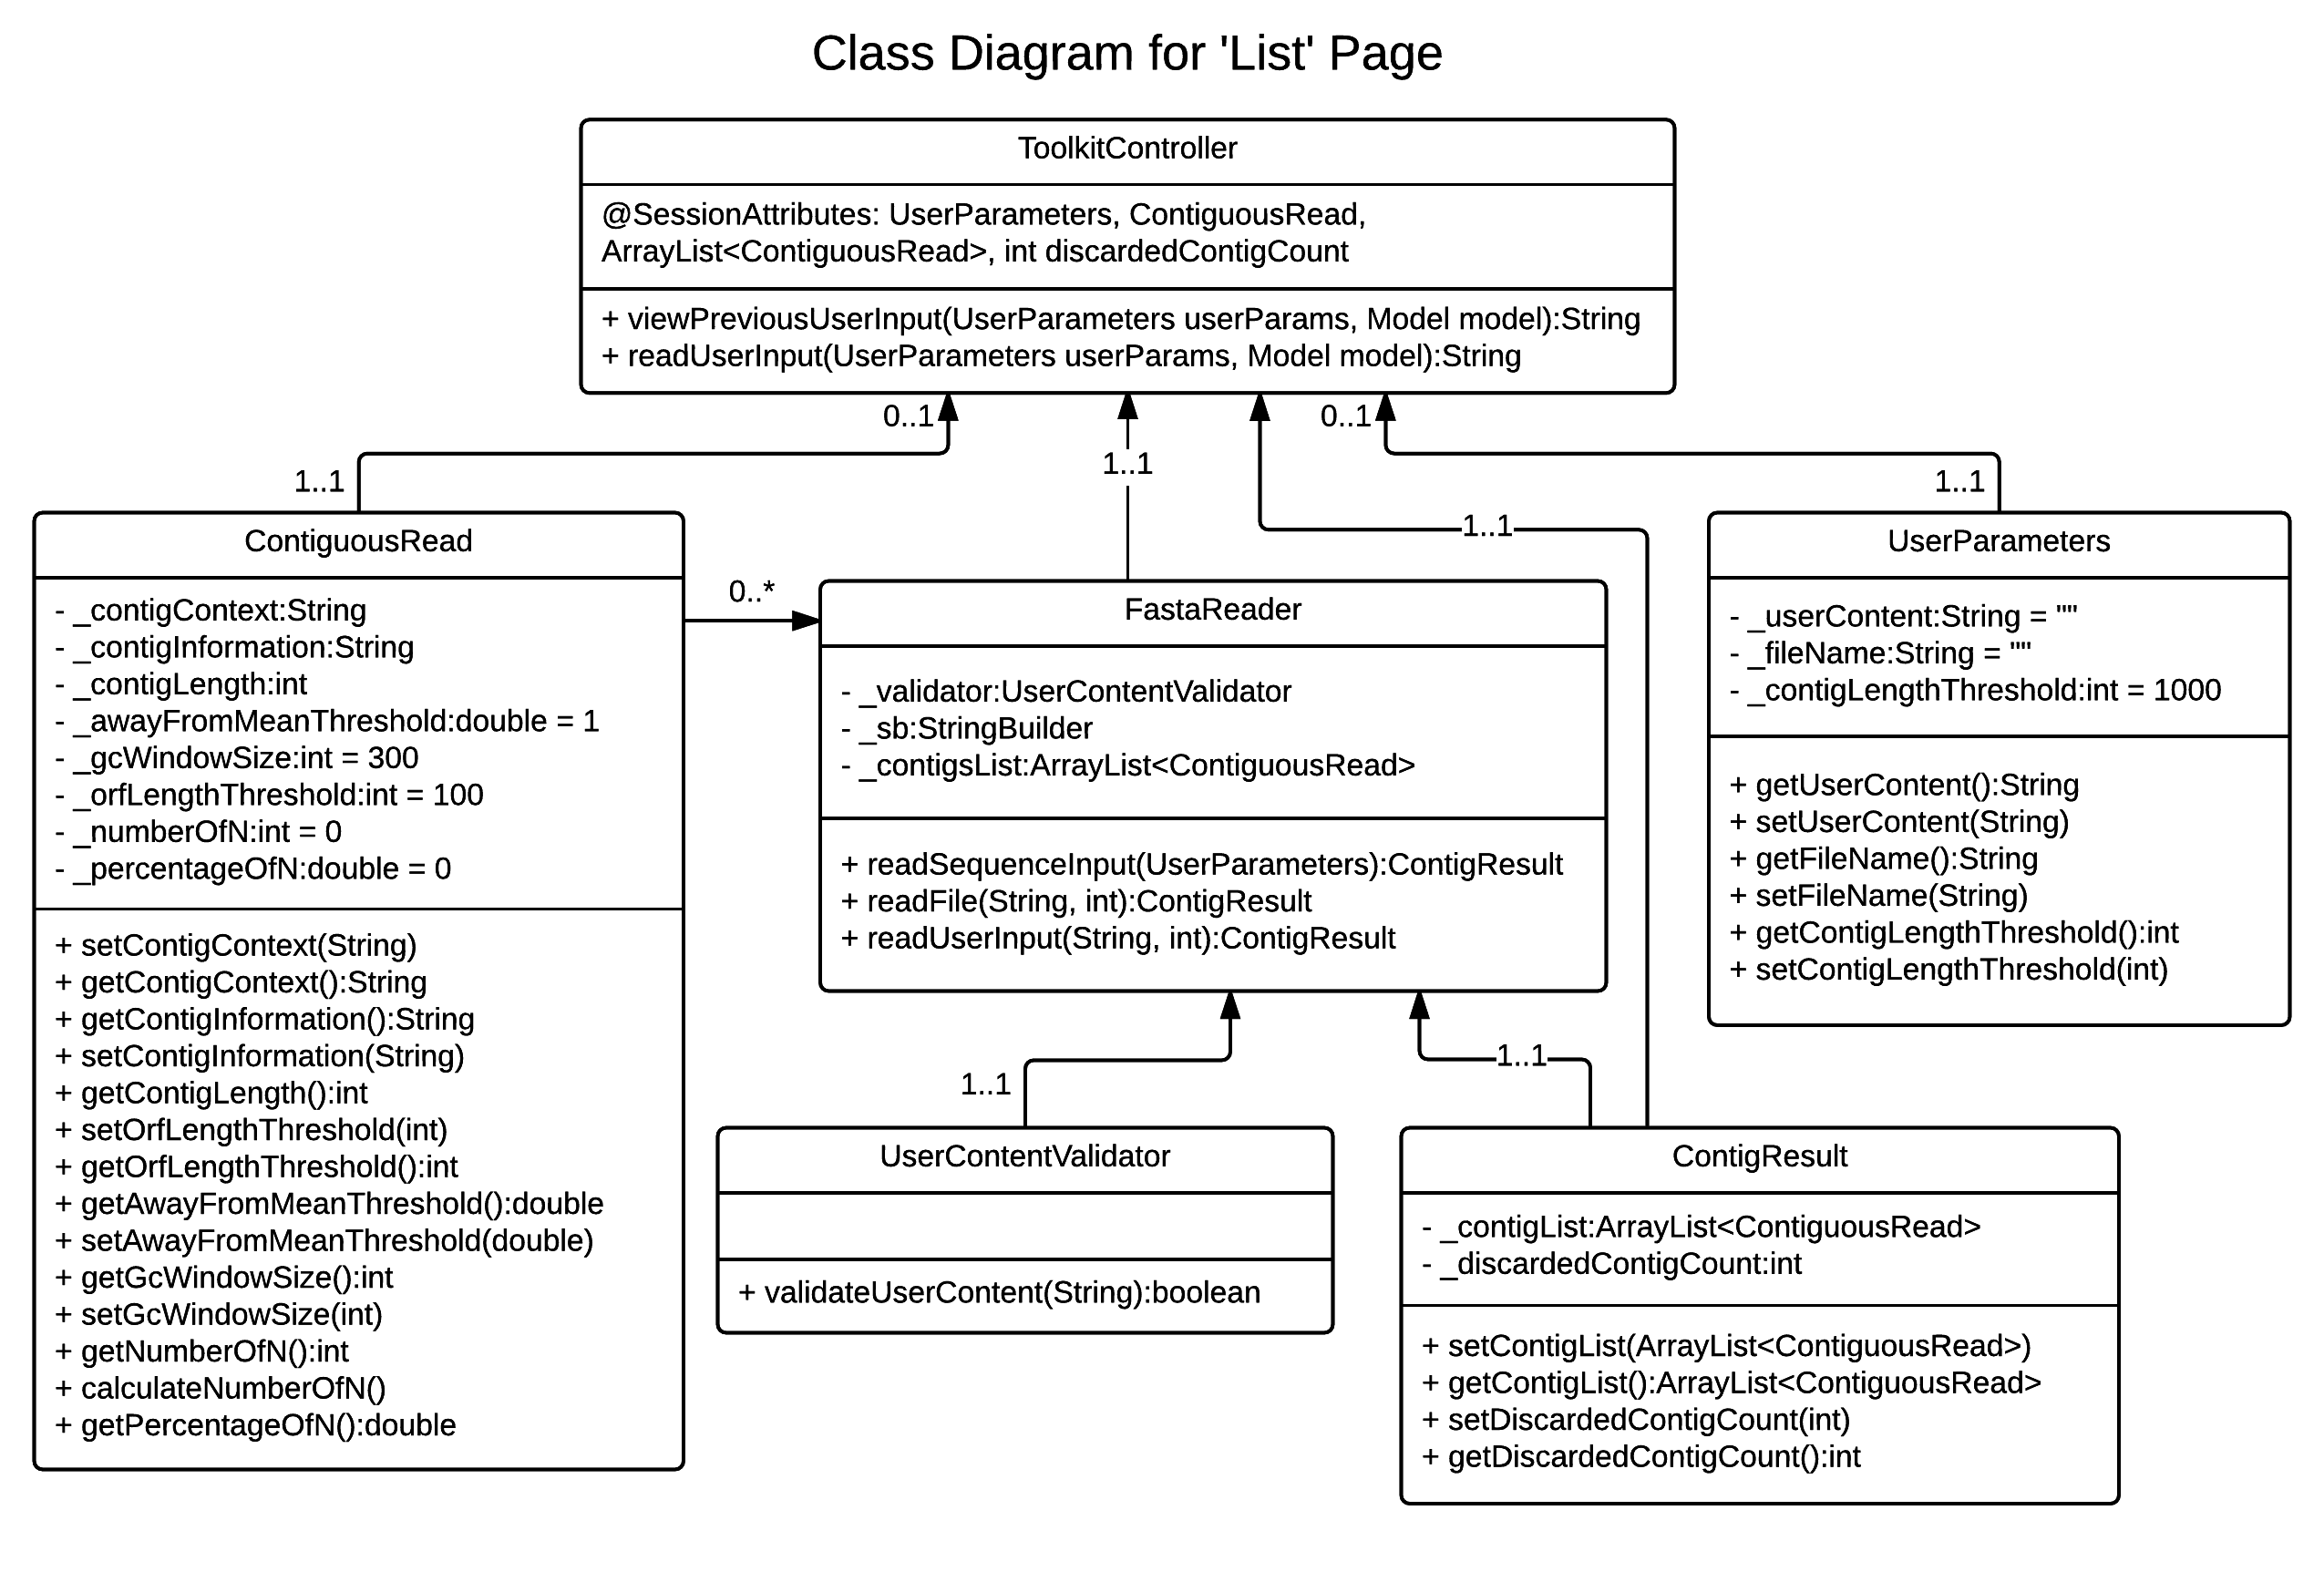
\includegraphics[width=0.8\textwidth]{images/umllistpage}
\caption{Class diagram for the `List Page', and what classes are used upon a Request for the page.}
\end{figure}

\begin{figure}[H]
\centering
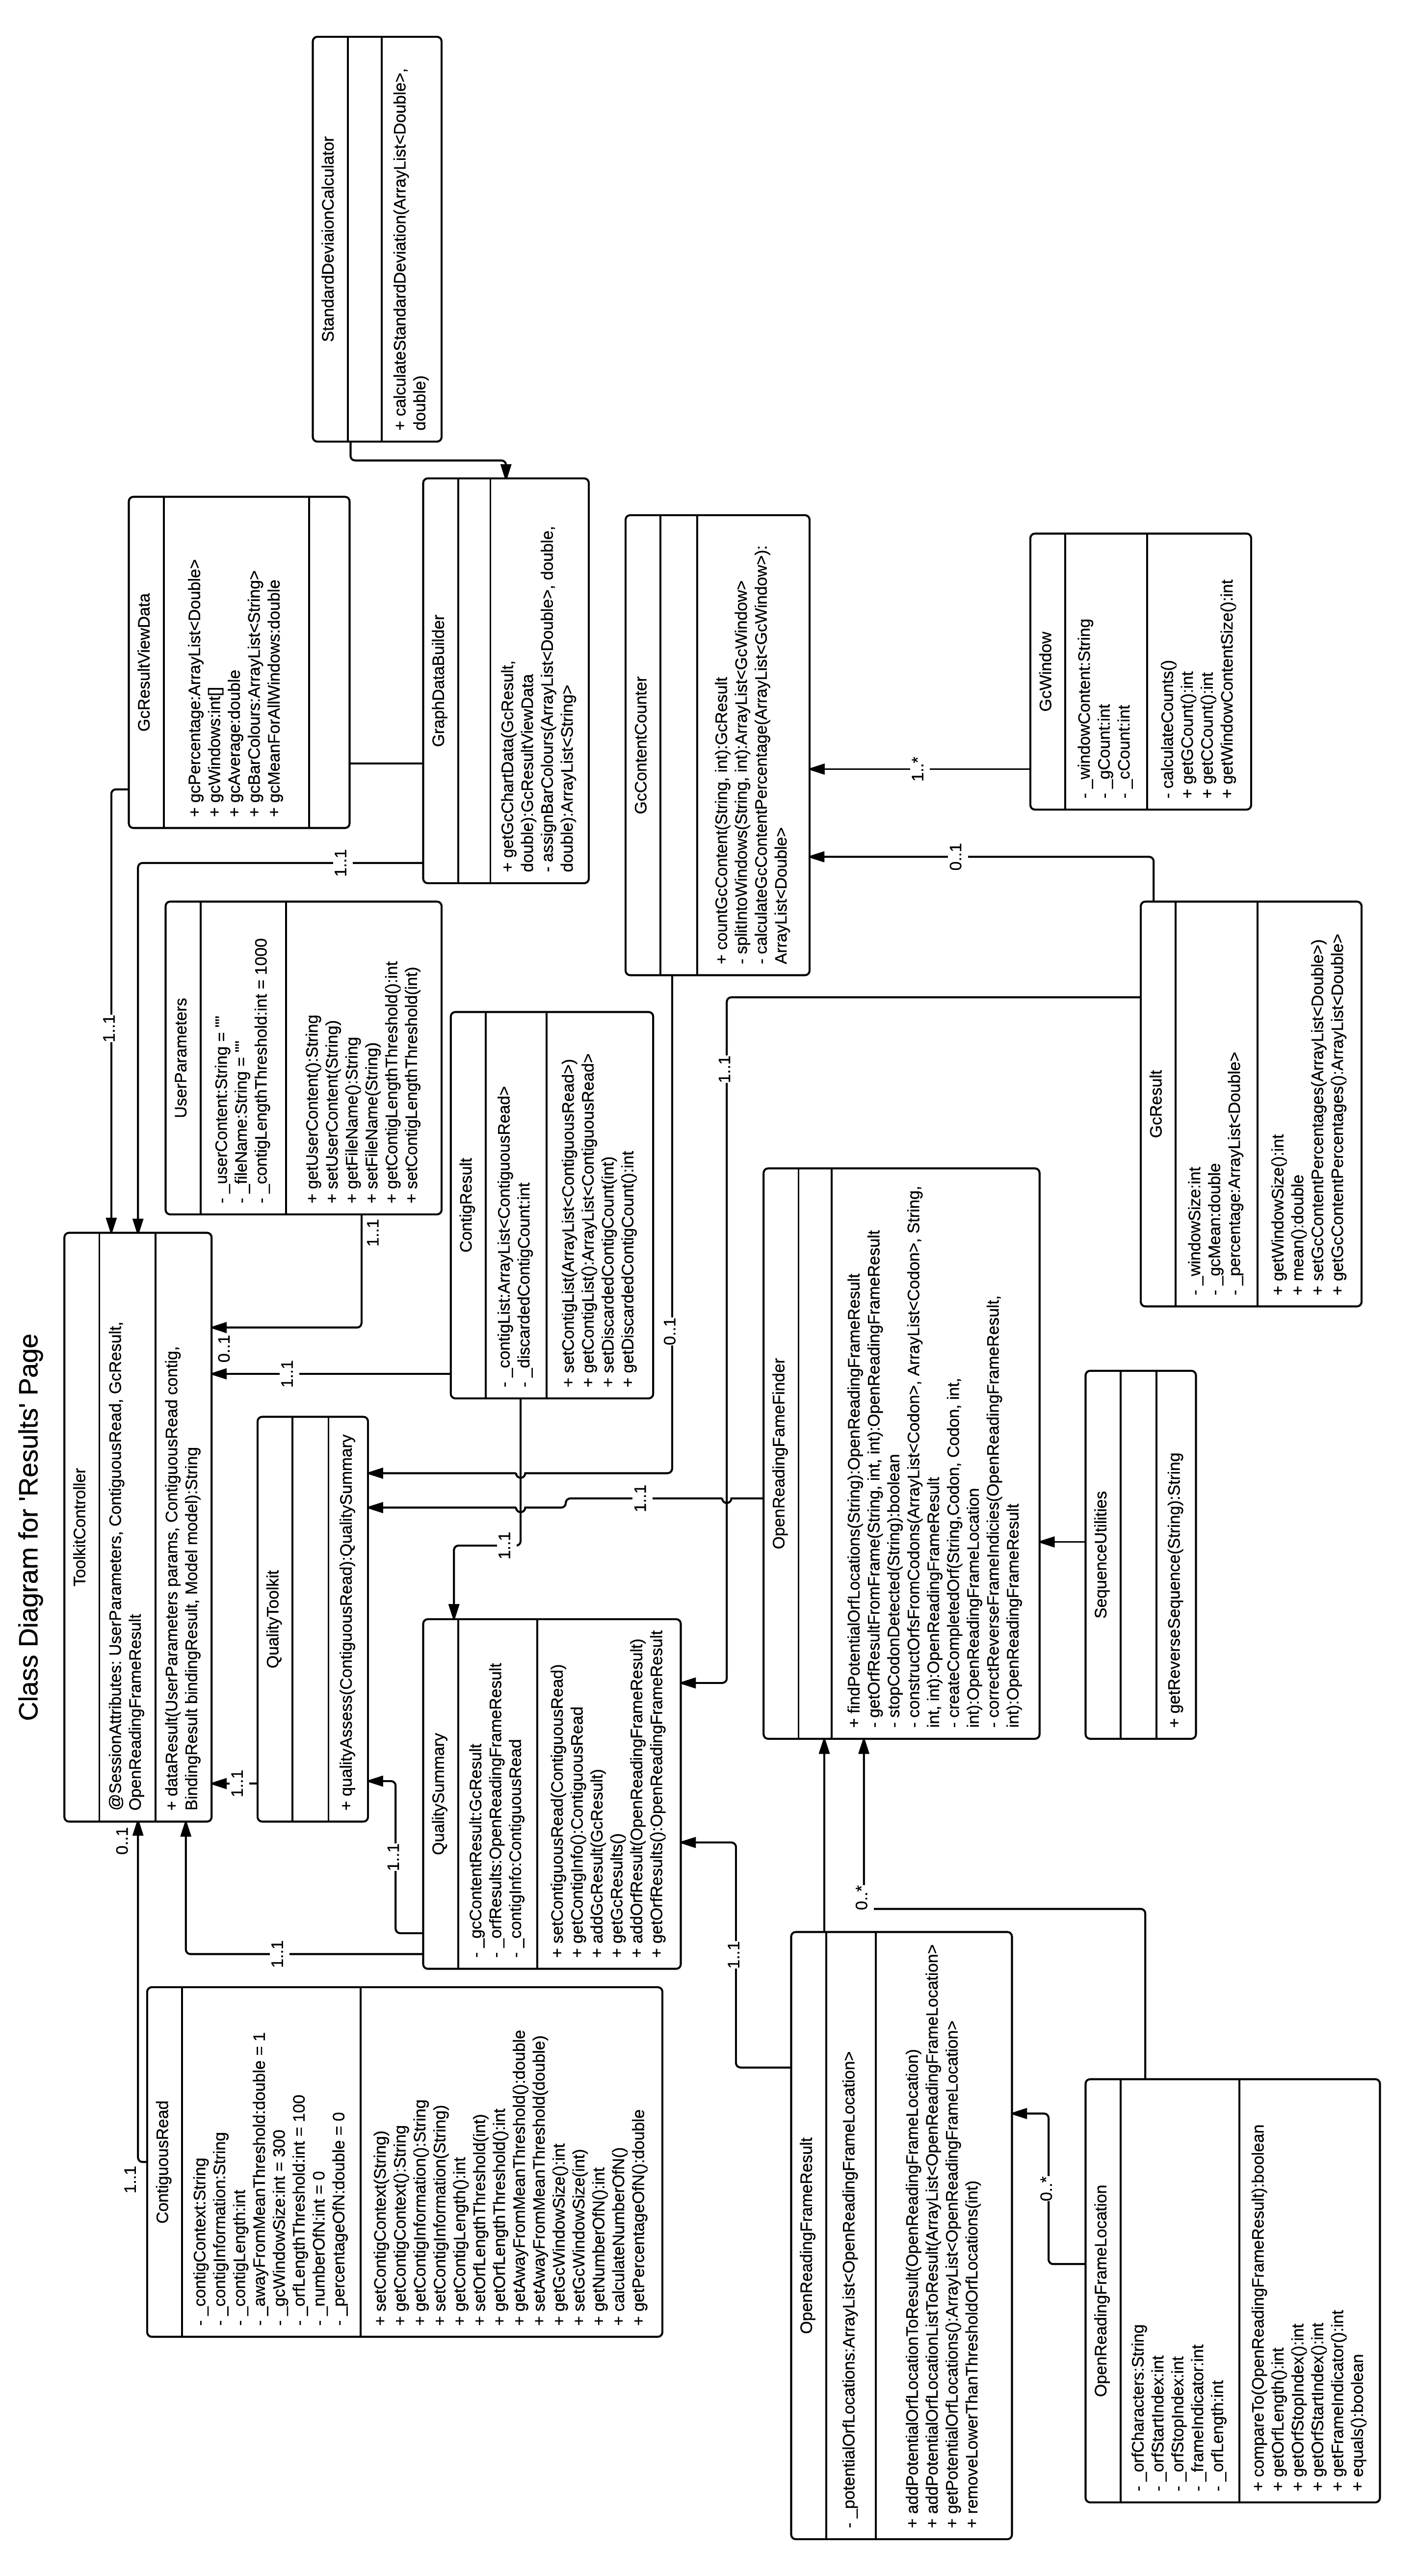
\includegraphics[width=0.8\textwidth]{images/umlresultspageflip}
\caption{Class diagram for the `Results Page', and what classes are used upon a Request for the page.}
\end{figure}

The structure evolved over time due to the nature of XP and using an agile methodology. Even so, the result was that there was a logical sense to the structure of classes, methods belong in the class they live in, some utility classes exist for carrying out operations that don't necessarily need to be within a class that needs that utility and this also left the code easier to maintain and separated. By using utility classes and methods, they can be called by other classes in the future, and the class that uses them doesn't need to know about the implementation internals of the methods they use, only the results.

\subsubsection{View}
The View of the application is where the GUI is presented to the user to be seen in their browser. Designing the application to use the browser was chosen to allow anyone to be able to use the application as long as they are using a modern browser. It is using HTML, HTML5 Canvas and JavaScript, dynamically built using Thymeleaf templates. If any of the template does not process or there is an issue with the users data they are presented with an error page and told to return to the menu and try their task again.

The data for the View comes from the Model, passed by the Controller. In line with keeping responsibilities separated, the Model does not care about how the View displays the data, and the View does not care about the content of the Model data it is passed as long as the data types it expects are present in the Model from the Controller. For example, the ORF Location data is sent to the View as an OpenReadingFrameResult Object, that has a list of OpenReadingFrameLocations and other data about the process. It is then the responsibility of the View to use this data in displaying it in HTML5 Canvas with JavaScript. No additional processing or modifications are carried out on the data at this point, the View just picks up the data and places it on the Canvas element where it expects it should go, based on the content of the data, e.g. an OpenReadingFrameLocation with the `frameIndicator' set as 0 would indicate to the View that it should be placed on Frame 1.

This type of responsibility separation is consistent throughout the application, with one exception. There is a GcResultDataView, that is the GcResult data processed into an easy to handle class. This is to make the process for the View far faster than having to get the View to carry out some processing to determine the GcWindows that are out of the mean threshold and additional results to display on the bar chart for the GcResult. While it would be possible to alter the application in order to leave this up to the View, I felt that it would be better to instead serve the View with the window data it needed to put on the chart and the colour codes for each of those window data bars. If the View for this result were to change in the future, no additional processing would be required within the Model to match this, as the results are still present in their raw form for the View to use as it sees fit, and so I felt this was an acceptable design choice.

\subsubsection{Controller}
The Controller serves as the master for how data flows through the application, making calls to methods from the Model to process the users data, receiving requests from the user via the View and HTML Requests and handling what data is used in the View. The user may send HTML Requests to the different pages of the application and will receive a response based on the `@RequestMappings' of the Controller. 

For example, a GET Request on the `list' page will return a page expecting the user to have already submitted some data that has been turned into a list of contigs. A POST Request on the `list' page however will be expecting that this is a new set of data and process the data submitted into a list of contigs and put them into the users session attributes.

Through every page, a user carries a Session with them and particular session attributes are expected at certain points in @SessionAttributes. For example, a user must have UserParameters and a ContiguousRead in their session parameters in order to be able to view the List and Results page. If they have not visited the Welcome page and submitted data, however, it is not possible for them to have these attributes, and so they are locked out of those pages. This is good behavior as the user should not be able to try and view results for data they have not submitted.

\subsection{Naming Conventions}
I followed a naming convention of attempting to name classes, methods, fields and variables in such a way that a reader could understand what the function of that particular thing was just from the name alone. Private field names all begin with an underscore, e.g. `\_privateField' and everything is written in camel case, starting with a lowercase character, e.g. `thisWouldBeAMethodName()'.

\subsection{User Input}
Based on the background reading, the decided file format to accept was FASTA format. The design allows for user uploading and user pasting of files in the Model methods. However, in the end I decided to keep the design just to handling pasting of data. This was based on a time constraint and issues with file upload limits, security and the need to test. While the functionality has been left in the code, it has been left as a `if I were to continue' functionality to be expanded upon if I had more time to work on file uploading as a priority over different techniques for the quality assessment.

User data is also not kept by the application, it is stored in a user session that expires once they leave the page. This is handled by Java Spring, and set as one of the @SessionAttributes. If the user does not have their session variables, they are presented with the Error page, so they cannot try and access areas of the application/web service where they currently do not have access or the data to do so. This means that the data they have is their own, and not retained by the application or possible for other users to access.

\subsection{Directory Structure}
The directory of the applications structure was designed such that it would reflect the MVC aspect of the application, and make finding resources and particular Classes easier for a reader. The design makes the application easier to maintain in the future and is another way of helping to enforce separation of responsibilities between classes and resource types. In the figure below you can see the way that the directory structure is designed to back this up.

\begin{figure}[H]
\centering
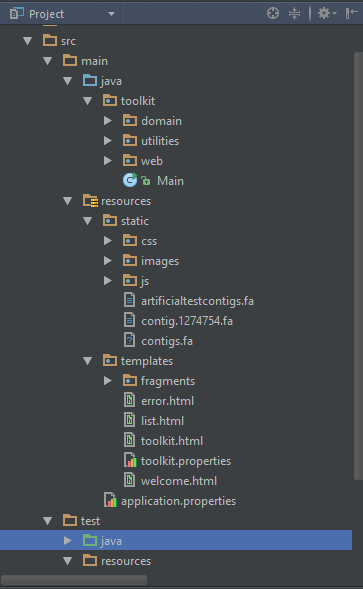
\includegraphics[width=0.5\textwidth]{images/directorystructure}
\caption{The layout of the directory structure for the application.}
\end{figure}

Within the `src/main/java' folder, there are the sub folders `domain', `utilities' and `web'. Separating the classes out this way helps with the previously mentioned separation of responsibilities. Domain contains the classes for the domain objects themselves and the data and processing (the Model, so GcResult, OpenReadingFrameLocation, etc), Utilities contains utility classes for use by any of the other classes and to allow their functionality to be independent of any domain class and Web contains the Controller classes (ToolkitController, ErrorController).

\subsection{QualitySummary and Results}
In the application, the quality assessment results are returned in a QualitySummary object. This QualitySummary contains references to GcResult and OpenReadingFrameResult. There is the option to have these two implement an interface that might be called QualityResults, and have just an array of QualityResults in the QualitySummary rather than defined result types. This would allow us to add any type of result without needing to know what is in there. However, I chose not to do this as considering the way in which we serve data to the View it seemed okay to be able to have the View called results from the model directly, and through XP developing this any further would go against YAGNI. 

I am aware that in the future if a user was allowed to select what type of processing they wish to use and as more techniques for quality assessment are added, this technique would be very useful to implement. It would be possible to do this and in the View have it check for the existence of the expected results, or check if they were empty/null, and then only dynamically include fragments of results that are present. 

\section{User Interface}
Below is the finalized designs of the user interface, shown through screen shots, along with an explanation for the design choices in how the pages are laid out for the user to navigate through. Each page has a header, containing the title of the application and the logo I made. 

The logo is based on the mythical creature `chimera', a creature made from multiple parts of other creatures (often a lion, snake and a ram). The inspiration for the name and design comes from the application hoping to highlight potential Chimeric regions of contigs to a user, hence `Chimera - Metagenome - Chimeta'. The `K' in Chimera is simply because `Chimeta' sounds too much like it would be pronounced `chai-meta' not `kai-meta' as in `kai-meera' for Chimera. It isn't an important aspect of the design.

% ==== Welcome ====
\subsection{Welcome}
\begin{figure}[H]
\centering
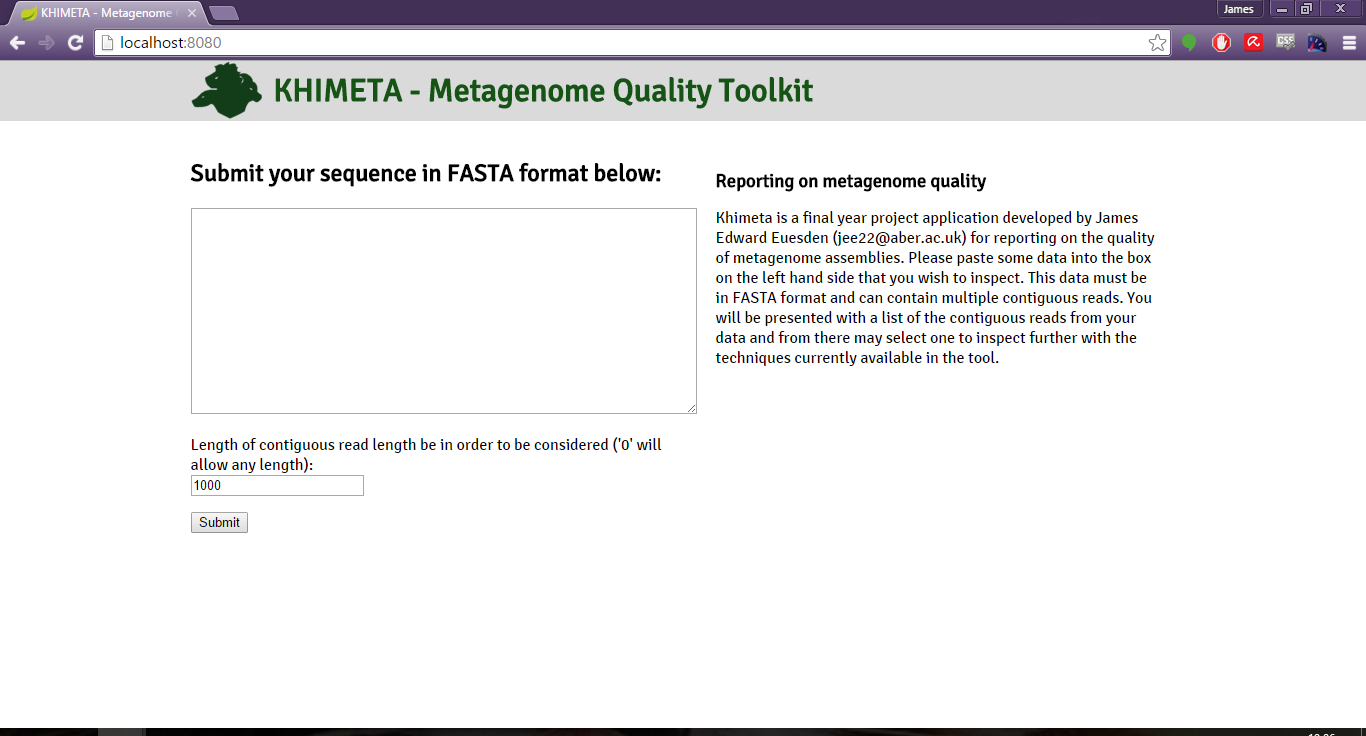
\includegraphics[width=0.8\textwidth]{images/ui1}
\caption{The `welcome' page that greets the user upon requesting the home page of the web service.}
\end{figure}

The welcome page is structured so that there is an explanation for the user of what the tool is, and an area for them to paste their FASTA data in. There wasn't much else needed for this page, but were the project to be continued this is where there would also be the option to upload user files instead of pasting in data. The user also specifies the minimum length a contiguous read must be in order to be considered here.

The original design for this page also included the parameters for modifying the quality assessment, as this tied in with when the application dealt with only one contiguous read at a time. As the application evolved, the design changed and was refactored to shift the parameters for quality inspection to the next page where they could be tied to contiguous reads and not to the assembly data submission as a whole.

%==== List =====
\subsection{List}
The below images show the `List' page, where a user can see all of the contiguous reads within their uploaded data file that are above the minimum length threshold they specified. The page also displays the number of discarded contigs due to the length, as I felt this would be useful information to give to a user.

For each contig, I also believed it would be useful for the user to see the contigs header (name), the length (how many characters) and the number of unknown `N' characters, along with the percentage of those that made up the contig. This could be used for a user to consider whether a contig has too many of these characters to the point that they feel it is a bad quality contiguous read.
\begin{figure}[H]
	\centering
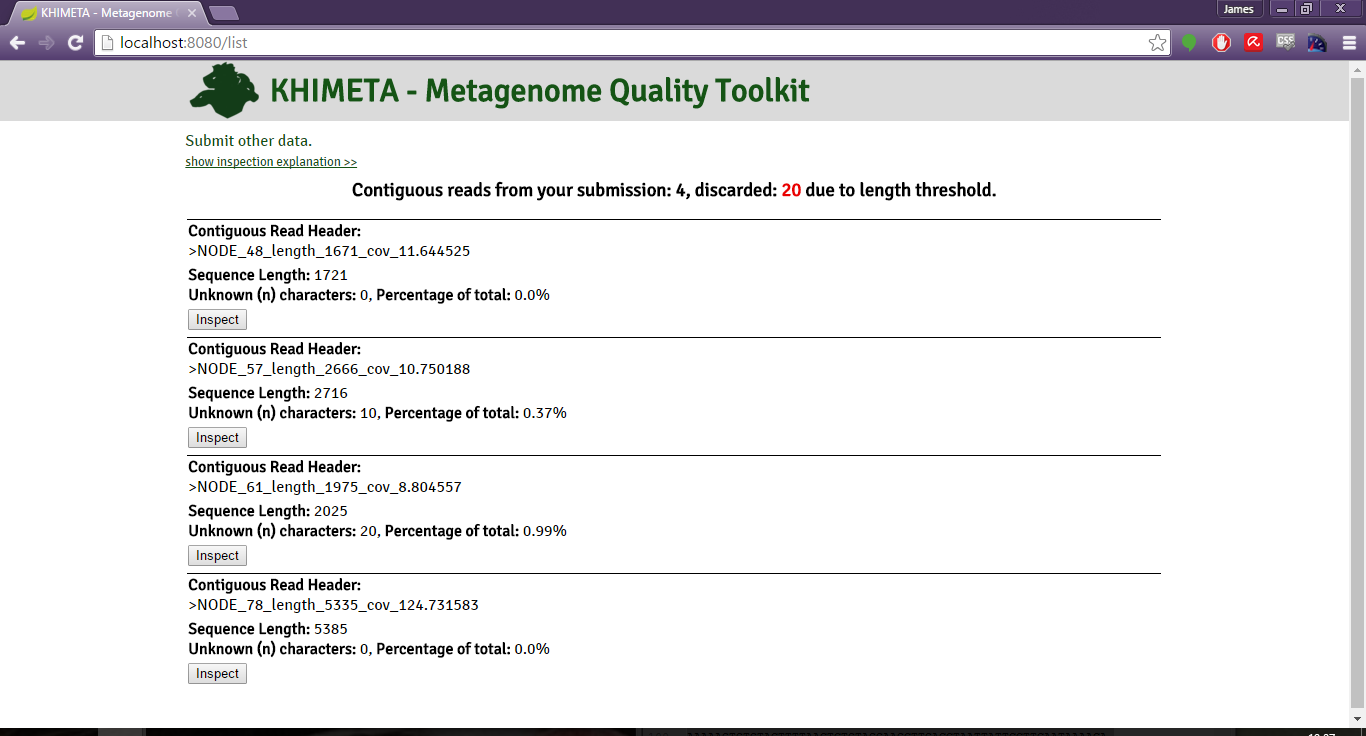
\includegraphics[width=0.8\textwidth]{images/ui2}
\caption{The `list' page that is displayed after a user submits their (valid) assembly data in FASTA format.}
\end{figure}

If a user wishes to further inspect a contiguous read, I designed it such that when they click to `Inspect' on a contig, a box appears underneath the contig information for them to modify the parameters for the quality assessment process. I had previously considered a design where these parameters were on the right side of the list, and would stay static there as the user scrolled down the page. However, if a contigs name was very long it would run `underneath' the box and be hidden. I also found it just did not look very appealing, and so I opted for the design you can see below instead. When the user clicks to run the process the `Inspect' button changes to `Loading...', to inform the user that the process is working.

\begin{figure}[H]
	\centering
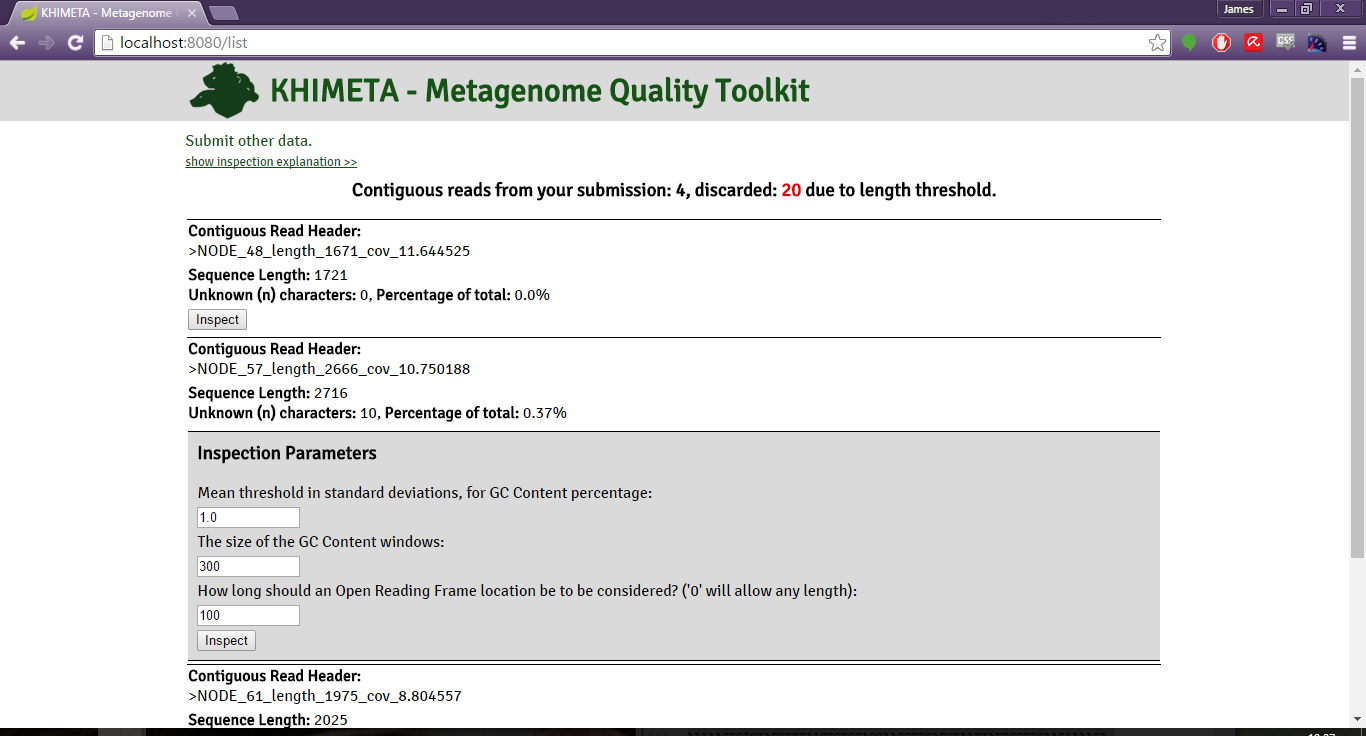
\includegraphics[width=0.8\textwidth]{images/ui3}
\caption{When a user clicks to inspect a contiguous read, this menu appears giving them options to alter the parameters of the quality assessment inspection.}
\end{figure}

In order for a user to understand what the inspection process is, I included a box that details the process, which appears when they click the words for `Show inspection explanation'. This box can be hidden by clicking the `Hide inspection explanation'. Currently, the link to display the explanation is at the top of the page, and a user must be at the top of the page to click and view it. It could instead be possible to have the list of contigs scroll in their own box, such that the inspection explanation is always available to be seen and viewed when clicked. However, it did not fall into scope of my Sprints while working on the functionality.

\begin{figure}[H]
	\centering
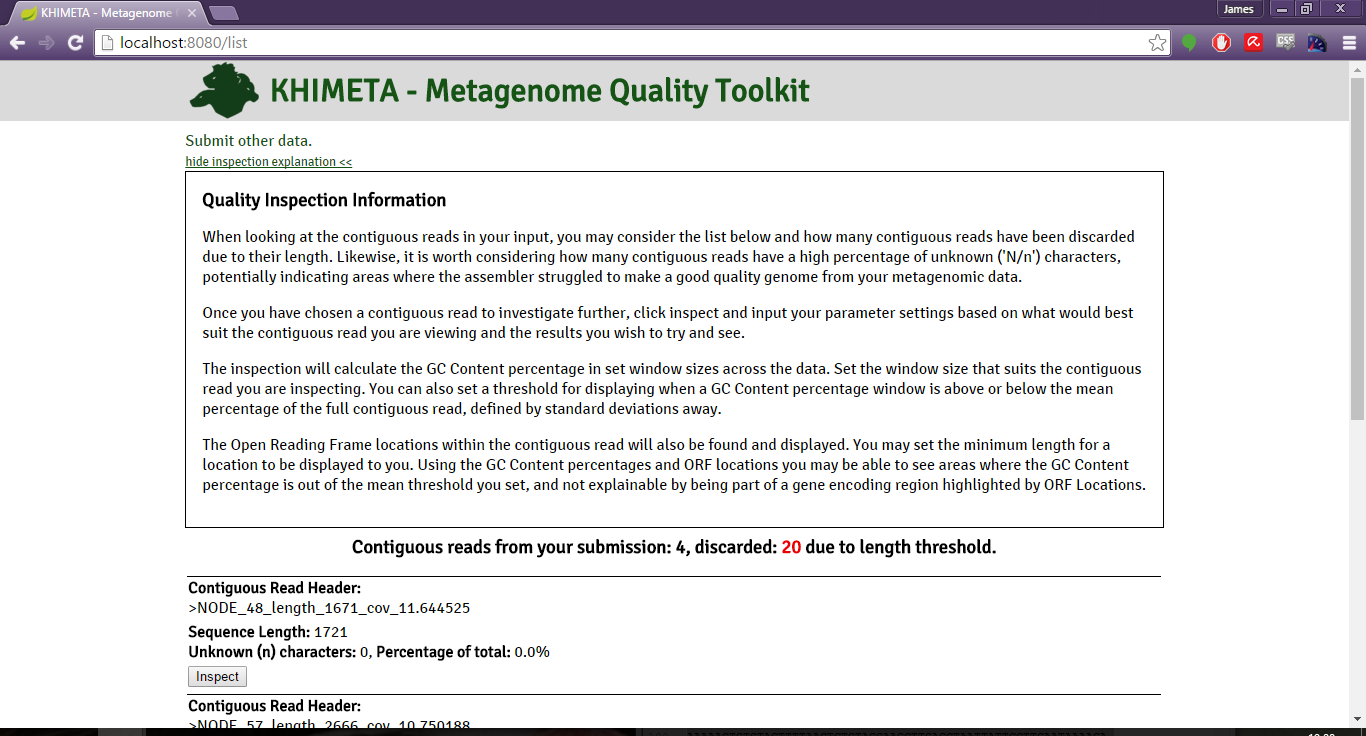
\includegraphics[width=0.8\textwidth]{images/ui4}
\caption{If the user clicks to see an explanation of the process, they can click the text that says to `Show explanation', and this text appears.}
\end{figure}

\subsubsection{Parameter choices}
The choice of parameters that the user can modify were selected based upon what could be altered about the inspection processes. For example, allowing a user to change the minimum length of an Open Reading Frame location gives them control over what size they think is important, based upon what their assembly data is. It could be that they care about any sized potential protein coding region, or that they only wish to see ones of size 1000 or above, as they know that anything less is unlikely to be an actual protein coding region. Giving them this parameter choice allows them to decide this for themselves, as the application won't know what is the best size for the user.

Similarly, the GC content window size should be set by the user, again based on what they think is a reasonable size. If a user were to think that they might want windows of size 100, that probably wouldn't return them great results on a large contig, as the GC content could vary so much between windows where the data is just too small to be useful. Likewise if the window size is too big, this data may also be useless, as they cannot properly compare their GC window sizes to the expected size of what they want to see from protein coding regions.

A reasonable window and minimum ORF Location size can only be selected by the user, and so the choice was made to allow the user to select their own choices, even allowing them to select values to high or too low, it is their decision to make based upon the data they have provided. In future versions of the application, it would be interested to infer a decent window size for the user and suggest it to them, but for the purpose of this project it was out of scope for the time allotted with the other functionality to be implemented.

The final parameter is how many standard deviations away from the mean of all GC content windows the user would like to consider is enough to warrant highlighting a window as being a potential issue. I selected standard deviation as it is a standard way of determining a value away from the mean that could be useful to inspect. Whether the user cares how much or how little this value actually is is irrelevant. The user may select what number of these they feel is useful to consider just for highlighting bars in the results chart.

%==== Results =====
\subsection{Results}
For the display of the inspection results, the user is shown a set of labeled tabs, that correspond to the techniques used. It is designed this way so that more tabs can be added in the future as more techniques are set in the inspection process, and to keep the page from being too crowded with results that would require a large amount of scrolling. The code for making the tabs themselves work is credited to Catalin Rosu\cite{tabcode} and their original code can be seen in the appendices.

\subsubsection{GC Content}
\begin{figure}[H]
	\centering
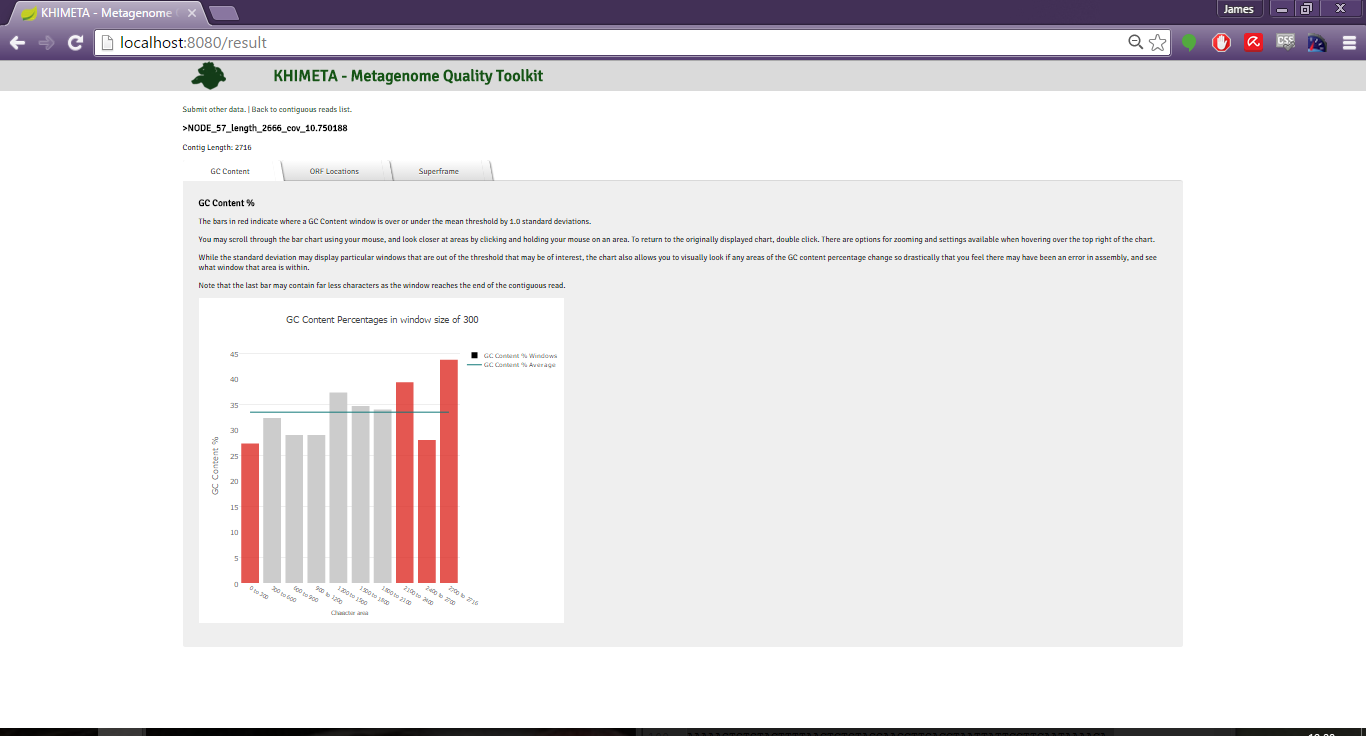
\includegraphics[width=0.8\textwidth]{images/ui5}
\caption{The GC result tab shown to the user on inspection of a contig. The browser has been zoomed out in order to display the page in full.}
\end{figure}

The GC Chart result is displayed to the user in order to give them a visual reference of how the GC content in their contig is. Through this they may detect single windows that may have chimeric properties through a difference in GC content above or below the mean, which can be highlighted in red and are set by being a number of standard deviations away from the mean. It also allows them to look and see if there is a naturally large difference at points between the GC content windows that are not necessarily picked up by the threshold.

The chart is built using Plotly.js\cite{plotly}, as it allowed me to give the user more control over how they view the GC content results in a chart than if I spent the time implementing my own solution to give them the same amount of fine-grained control. A number of the options offered to a user by the Plotly.js chart are probably far more than they need to be and may be confusing to a user. If the project were to be continued it may be worth developing a chart system for displaying the GC content without using Plotly.js, which could also help with developing a way of showing when there are drastic changes in the GC content not caught by the threshold.

Above the chart is a small explanation of what the chart is displaying, and what the user might look for in order to understand the chart and whether there could be potential issues in their contig displayed by these results.

\subsubsection{Open Reading Frames}
The tab for the Open Reading Frame displays a graphic made using JavaScript and HTML5 canvas, that gives the user a visual representation of 6 frames of the contig and any protein coding regions within those frames. The design was inspired by NCBI`s orffinder\cite{orffinder}.

\begin{figure}[H]
	\centering
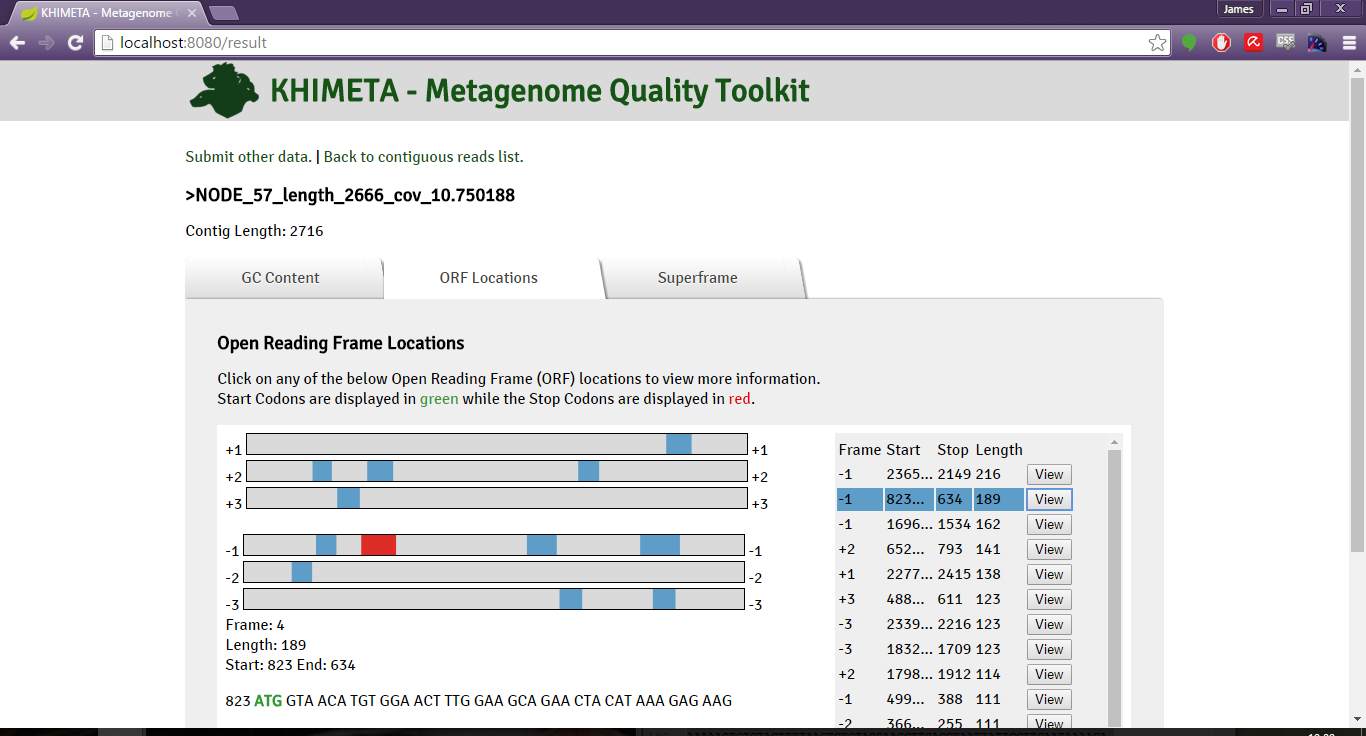
\includegraphics[width=0.8\textwidth]{images/ui6}
\caption{The Open Reading Frame results view tab.}
\end{figure}

I designed it in a way that allows the user to view the full list of ORF Locations (protein coding region) on one side, including their character length, start and stop point and which frame they are in, organized by largest to smallest. This is reflected in the frame chart where a user can see where the frames physically lie within the contig. If a user clicks an ORF Location, either on the chart or in the list, it highlights that ORF in the list in blue, and red in the chart. This also displays more information about the ORF Location underneath the chart.

The choice to display the ORF Location information was out of interest to the user if they wish to use the tool to look at the protein coding regions. The information displayed about an ORF Location includes the length, start and stop point and the characters within the ORF Location. While these might not be useful to the user for determining quality, the information is used in the comparison for GC content to find if the GC content is explained by an ORF Location, and so I believed the information might be useful to display to a user either way.

Each frame has its own canvas element, and they are aligned using a HTML table. I tried a design where each of the 6 frames was made up in a single canvas, and while this worked, it restricted the amount of formatting that could be done around each frame and had much more code for detecting whether a user has clicked within a frame, delaying the response a user got when clicking.

\begin{figure}[H]
	\centering
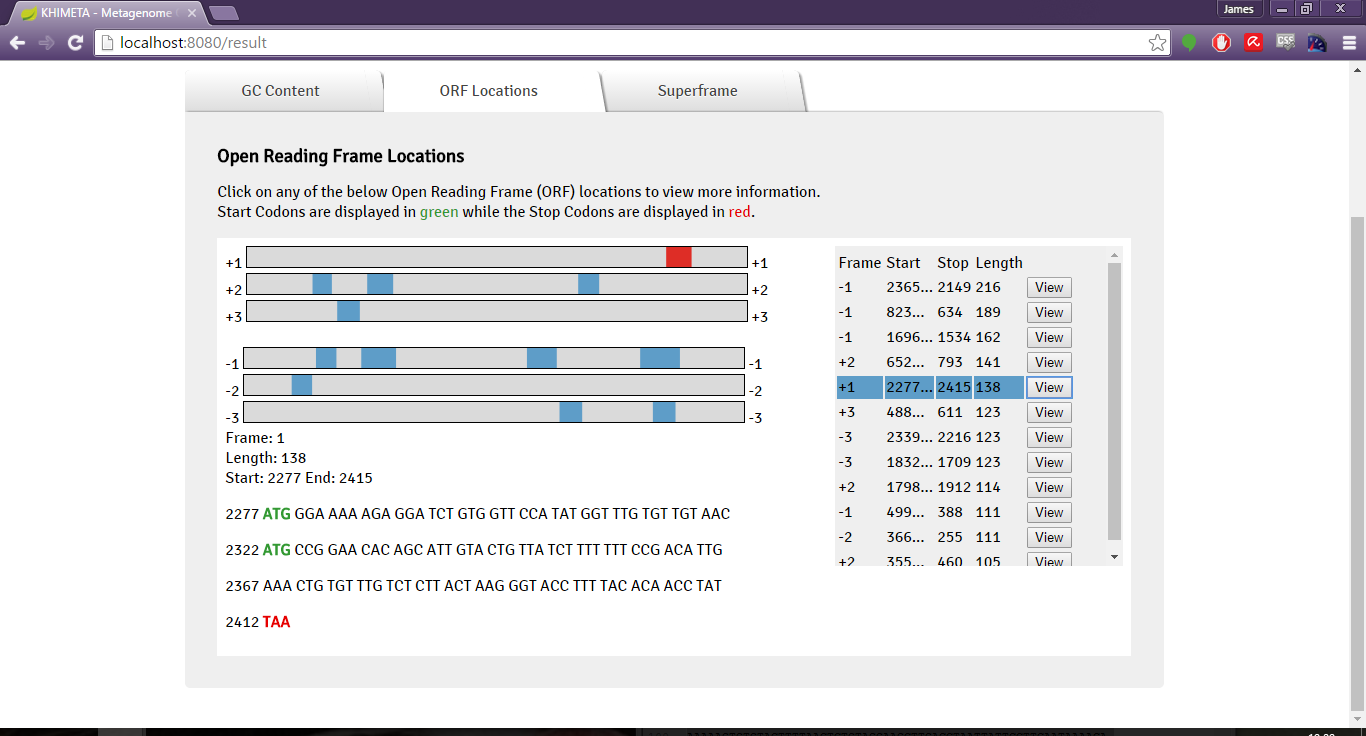
\includegraphics[width=0.8\textwidth]{images/ui7}
\caption{The Open Reading Frame results view tab, displaying that when a user clicks on a different ORF Location, the highlight on the frame chart and list changes to reflect this.}
\end{figure}

\subsubsection{Superframe}
Superframe is where the GC content and ORF Location charts are compared in order to help a user see if there are any areas of GC content difference that might be explained by the ORF Location. It is simply an overlaying of the 6 frames into one chart (all in the same sequence direction) and overlaying the GC content chart results for each window.

\begin{figure}[H]
	\centering
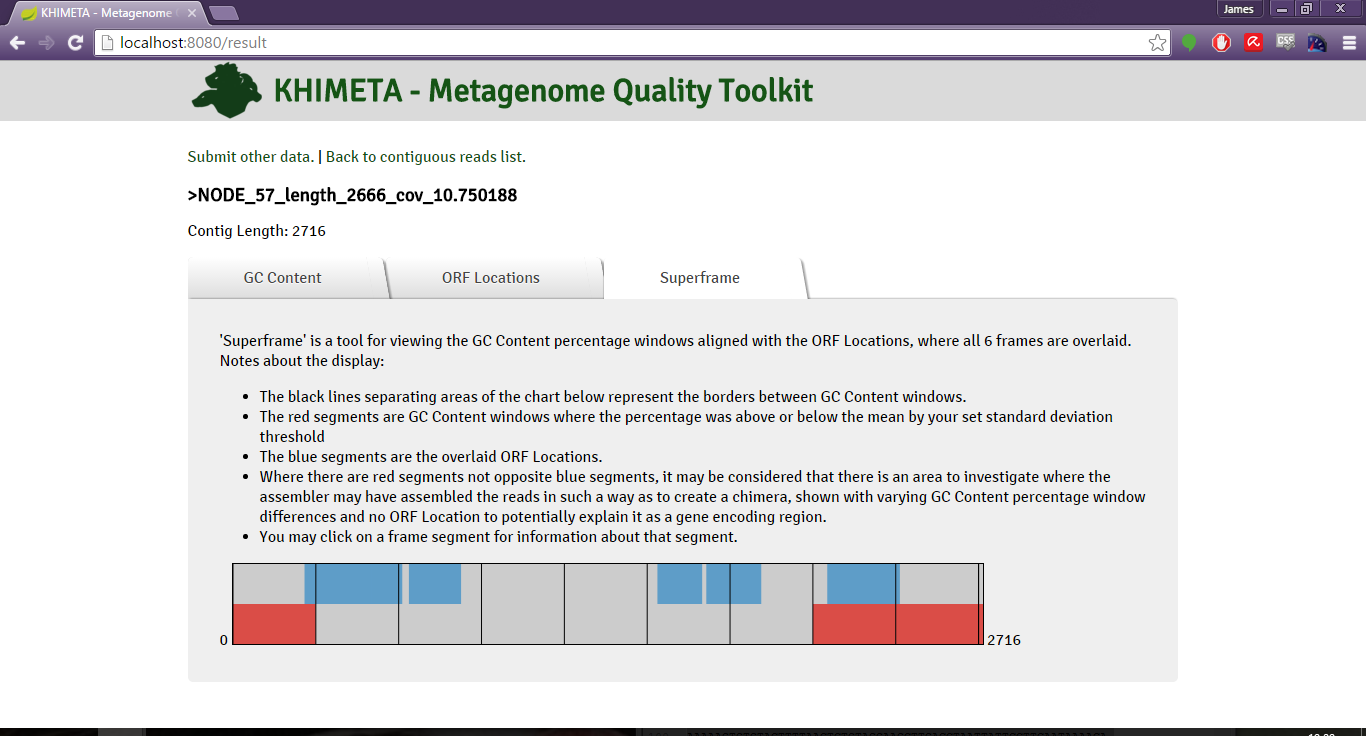
\includegraphics[width=0.8\textwidth]{images/ui8}
\caption{The `Superframe', a comparison between the ORF Locations within the contig and the GC content windows that are above the threshold..}
\end{figure}

If the user clicks on a particular window, they can see information about what window that is (where it starts and ends) and the GC content percentage. I felt this tool could be useful for a user to be able to determine themselves if they felt there were enough individual windows of GC content that were out of the mean threshold and not explainable by ORF Locations and so felt the quality of the contig was or was not good. I attempt to explain this with the description above the chart.

It is worth noting, the GC content areas highlighted for the Superframe are only those that are above the threshold of the mean, not below it. This is because it is those areas that are above could be explained by an ORF Location, as the GC content tends to be higher in protein coding regions, and so there is no use in displaying the GC content windows out of threshold by being below, which cannot be explained by the ORF Locations.

\begin{figure}[H]
	\centering
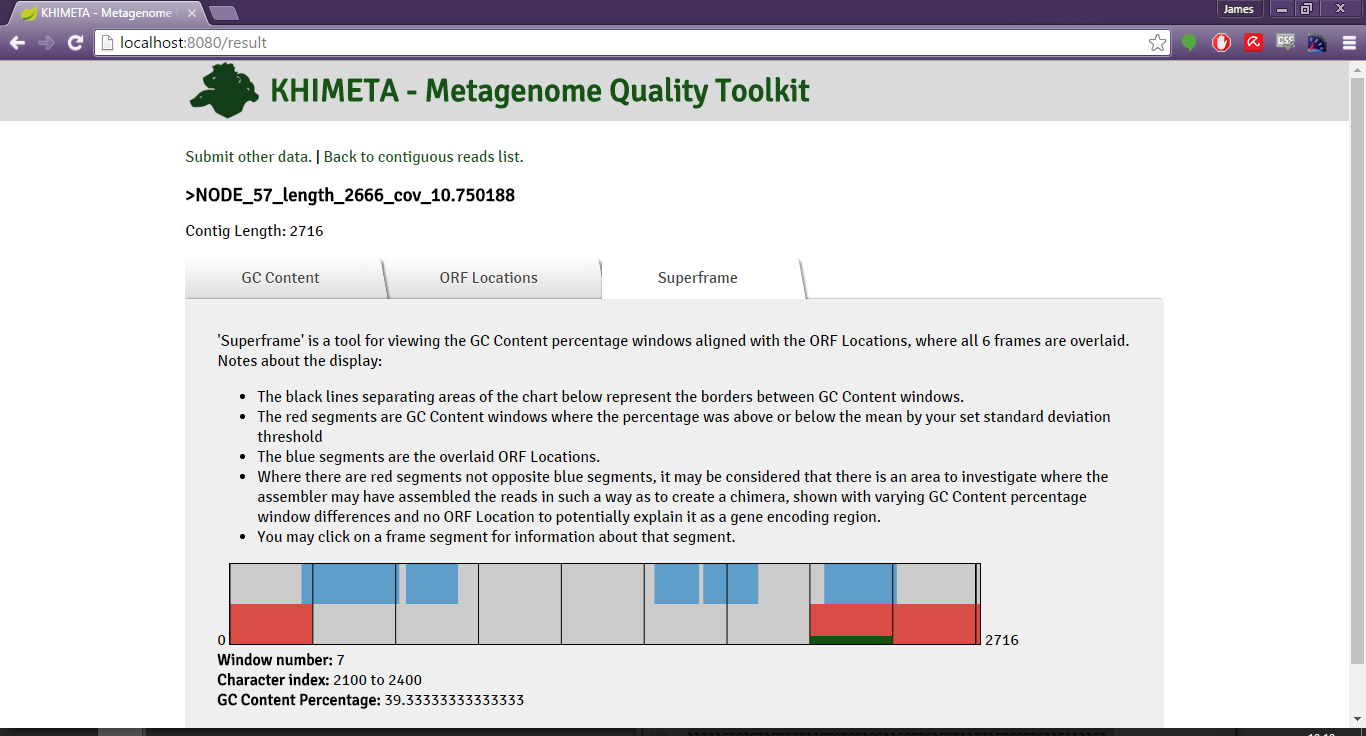
\includegraphics[width=0.8\textwidth]{images/ui9}
\caption{The result of when a user clicks to view a window data, they can see the particular percentage of the GC content of that window, and where that window starts and finishes, if they wished to inspect the contig themselves using those numbers.}
\end{figure}

%===== Error =====
\subsection{Error}
If a user encounters an error on the website, such as attempting to access pages without first submitting data) the page in the figure below will be shown.
\begin{figure}[H]
	\centering
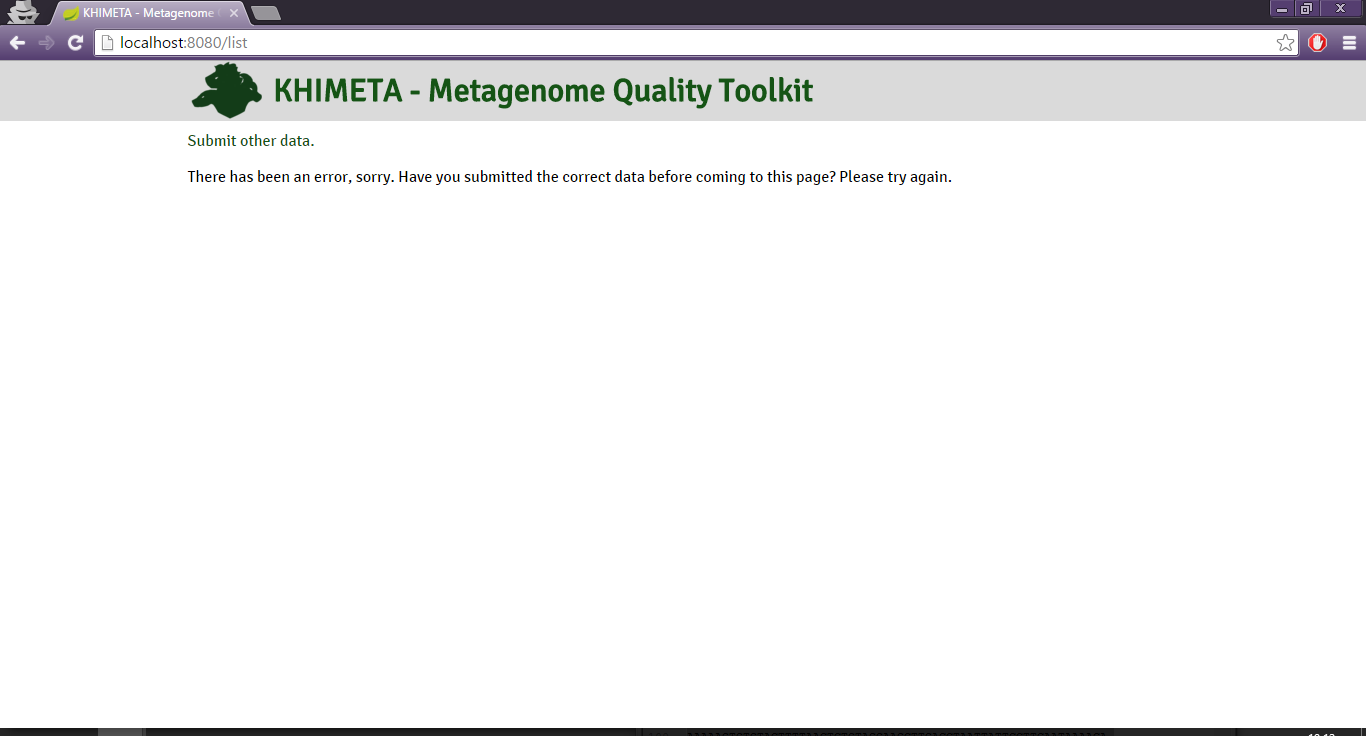
\includegraphics[width=0.8\textwidth]{images/ui10}
\caption{If an error occurs as the user is browsing the web service, i.e. they try to access a page when they do not have the required data submitted, they are presented with this page informing them of an issue.}
\end{figure}
While not very descriptive, it serves to return the user back to data submission, which is the best place to start again if something bad went wrong or they somehow tried to access a page when they hadn't previously submitted the required data. If there were a future revision of this page, it could be more descriptive of the exact reason why the error occurred, but was out of scope for the current project to make a fully detailed error reasoning. There is an ErrorController class in place however that can deal with this functionality in the future if the application were to be continued. Currently any errors are run through the Error controller but it only returns this page to the user.

\section{Support Tools}
For writing the code, I used JetBrains IntelliJ Community Edition IDE. This included writing all the code be it Java, HTML, CSS, Javascript, ThymeLeaf and any additional properties for setting up Spring. This was very useful for text highlighting, debugging the code, and tied into my version control, using Git and hosted on GitHub.

\begin{figure}[H]
	\centering
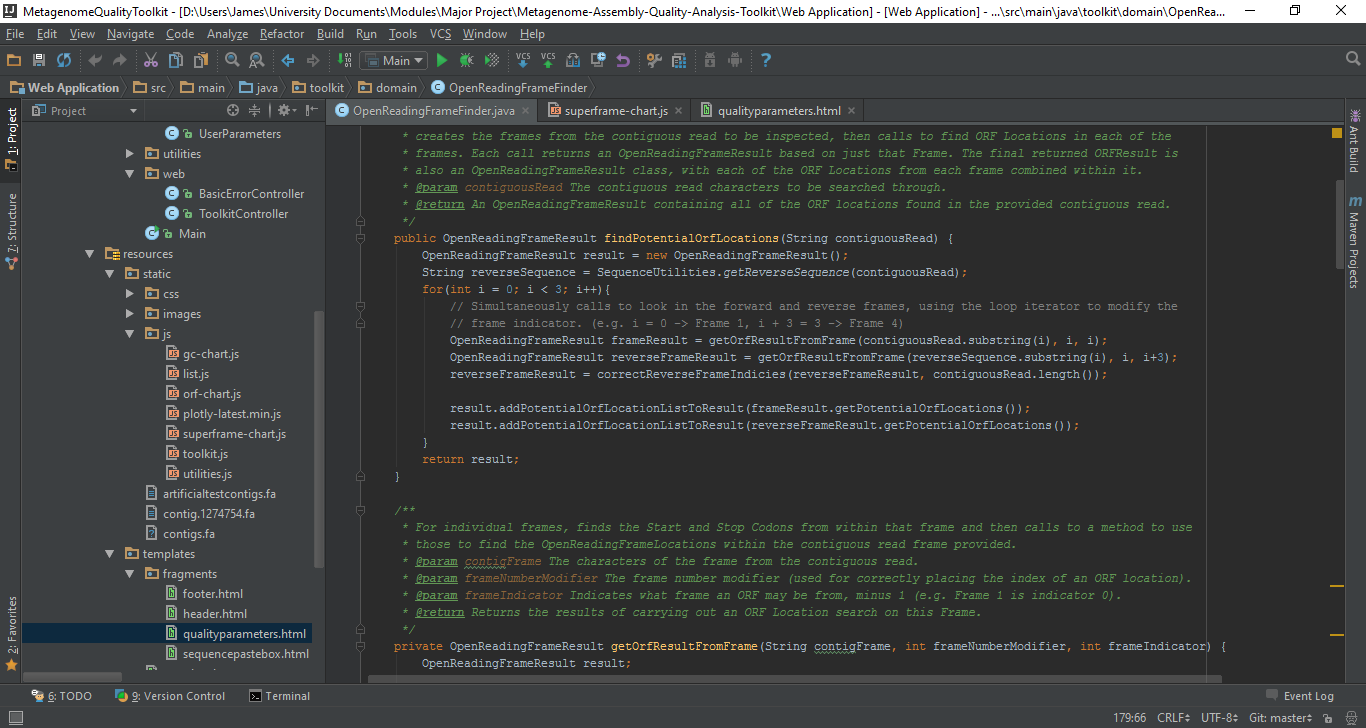
\includegraphics[width=0.8\textwidth]{images/intellij}
\caption{The Jet Brains IntelliJ Integrated Developement Environment (IDE) I used for developing my application.}
\end{figure}

I also used \url{http://www.tomato.es/} for counting my pomodoros. The web site provides a timer and a count for how many pomodoros have been completed during the time the browser has been opened.

\begin{figure}[H]
	\centering
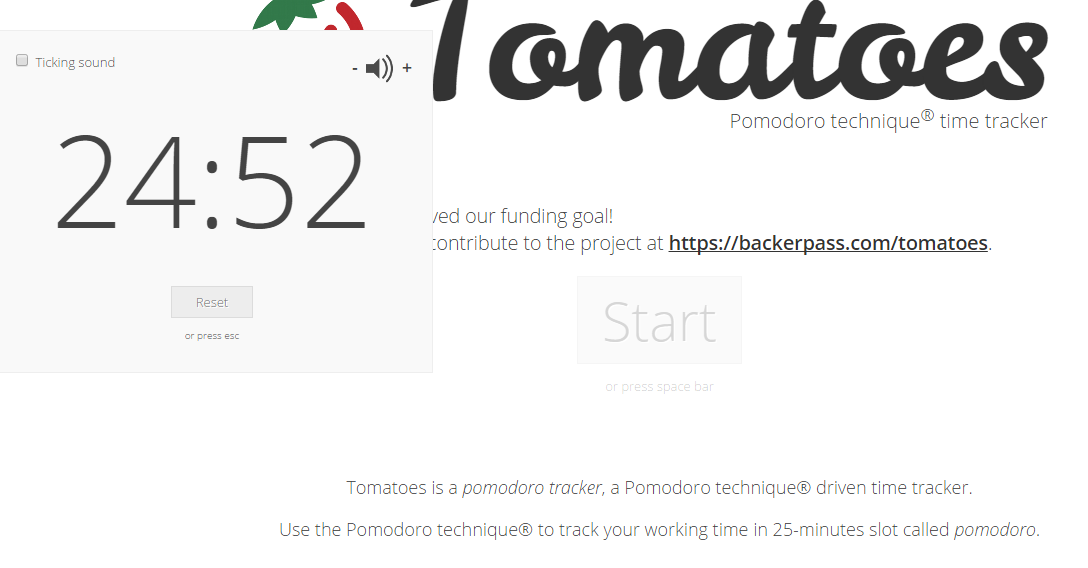
\includegraphics[width=0.8\textwidth]{images/tomatoes}
\caption{A countdown of the pomodoro tomato timer on \url{http://www.tomato.es/}, used for breaking up development time and keeping track of work done over time.}
\end{figure}

\subsection{Version Control and Continuous Integration}
I used version control to keep a repository of my code in case of losing data in event of hardware crash or software corruption. For this I selected to use GitHub as I already had a repository on there and Git is supported in the IntelliJ IDE I was using. This can be found at \url{https://github.com/coderghast}.

\begin{figure}[H]
\centering
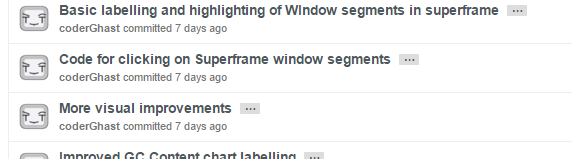
\includegraphics[width=0.8\textwidth]{images/commits}
\caption{A few of the commits made to my major project repository.}
\end{figure}

In addition, every time I checked in, I used continuous integration with CodeShip\cite{codeship}, allowing me to receive e-mails any time I made a commit to my repository that didn not pass the tests written. This was very helpful in discovering issues with failing builds when checking in a change and forgetting to update tests or breaking previously written code as the design changed.

\begin{figure}[H]
\centering
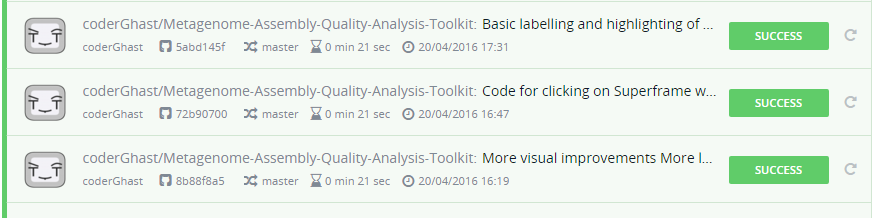
\includegraphics[width=0.8\textwidth]{images/codeship}
\caption{Examples of the continuous integration on CodeShip running my tests every time I committed to my repository.}
\end{figure}